%/*
% * SPDX-FileCopyrightText: 2021 Stefan Begerad <stefan@begerad.de>
% *
% * SPDX-License-Identifier: GPL-3.0-or-later
% */

\begin{frame}{Merkmale}
  Dede: eine freie, unabhängige und universelle Echtzeit-Karte
  \begin{itemize}
  \item FREI: Gemeinschaftsprojejt als freie Software (wie in Redefreiheit und NICHT wie in Freibier;-)) veröffenlicht\footnote{\url{https://github.com/dancesWithCycles/dede-front-end}}
  \item UNABHÄNGIG: weder ausgerüstete Fahrzeugflotte noch eigene IT-Infrastuktur notwendig
  \item UNIVERSELL: beliebige Fahrzeuge wie Bahn, Bus, Car-Sharing, Fahrdienst, Straßenbahn, Tram, Taxi, usw. universell darstellt
  \end{itemize}
\end{frame}

\begin{frame}{Integration}
  Mobilitätsanbieter erscheinen auf der Dede Echtzeit-Karte, wenn Ihre Fahrer oder Betreiber die Bewegungsdaten selbstständig erzeugen. Dazu brauchen sie nicht mehr als ein konventionelles Smartphone mit Internet-Verbindung und die Dede App.
\end{frame}

\begin{frame}{Dede Echtzeit-Karte}
  %alternative alignment to center is left and right
  \begin{center}
    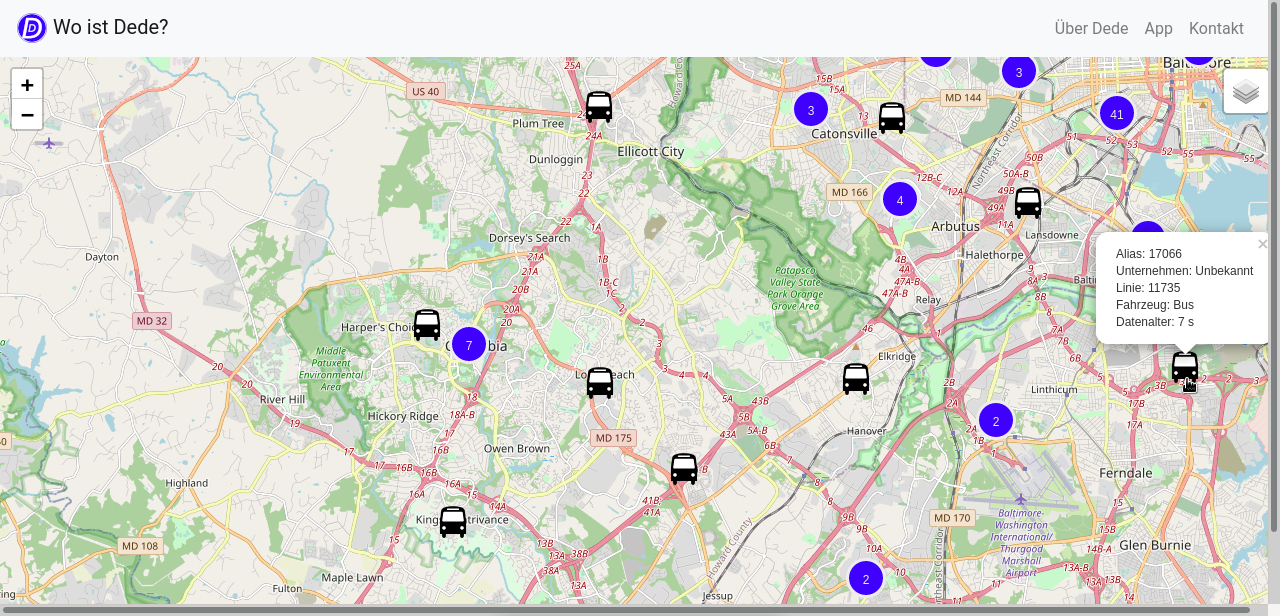
\includegraphics{dede/dede_real-time_map_crop}
  \end{center}
\end{frame}

